\title{Лекция 22\\Принципы многоагентной обработки баз знаний}
\author[]{Шункевич Д.В.}
\institute[]{Белорусский государственный университет информатики и радиоэлектроники}

\begin{frame}
	\titlepage
\end{frame}

\begin{frame}{\\Содержание лекции}
	\topline
	\justifying
	Понятие sc-агента, классификация sc-агентов. Принципы реализации многоагентной обработки знаний в семантической памяти. Спецификация действий sc-агентами, пример решения задачи коллективом агентов. Пользователь компьютерной системы как sc-агент. Спецификация sc-агентов, пример описания в базе знаний. Атомарные и неатомарные sc-агенты, иерархия sc-агентов.
\end{frame}

\begin{frame}{\\Понятие sc-агента}
	\begin{SCn}
		\scnheader{sc-агент}
		\begin{scnindent}
			\scnidtf{единственный вид субъектов, выполняющих преобразования в sc-памяти}
			\scnidtf{субъект, способный выполнять действия в sc-памяти, принадлежащие некоторому определенному классу логически атомарных действий}
		\end{scnindent} \vspace{5mm}
	Логическая атомарность выполняемых sc-агентом действий предполагает, что каждый sc-агент реагирует на соответствующий ему класс ситуаций и/или событий, происходящих в sc-памяти, и осуществляет определенное преобразование sc-текста, находящегося в семантической окрестности обрабатываемой ситуации и/или события.
	\end{SCn}
\end{frame}
\begin{frame}{\\Понятие абстрактного sc-агента}
	
	Предполагая, что копии одного и того же sc-агента или функционально эквивалентные sc-агенты могут работать в разных ostis-системах, будучи при этом физически разными sc-агентами, то целесообразно рассматривать свойства и классификацию не sc-агентов, а классов функционально эквивалентных sc-агентов, которые будем называть абстрактными sc-агентами. Под абстрактным sc-агентом понимается некоторый класс функционально эквивалентных sc-агентов, разные экземпляры (т.е. представители) которого могут быть реализованы по-разному.
	
\end{frame}
\begin{frame}{\\Классификация абстрактных sc-агентов}
	\begin{SCn}
		\scnheader{абстрактный sc-агент}
		\begin{scnrelfromset}{разбиение}
			\scnitem{неатомарный абстрактный sc-агент}
			\scnitem{атомарный абстрактный sc-агент}
		\end{scnrelfromset}
		\begin{scnrelfromset}{разбиение}
			\scnitem{внутренний абстрактный sc-агент}
			\scnitem{эффекторный абстрактный sc-агент}
			\scnitem{рецепторный абстрактный sc-агент}
		\end{scnrelfromset}
		\begin{scnrelfromset}{разбиение}
			\scnitem{абстрактный sc-агент, не реализуемый на Языке SCP}
			\scnitem{абстрактный sc-агент, реализуемый на Языке SCP}
		\end{scnrelfromset}
	\end{SCn}
\end{frame}
\begin{frame}{\\Классификация абстрактных sc-агентов}
	\begin{SCn}
		\begin{scnrelfromset}{разбиение}
			\scnitem{абстрактный sc-агент интерпретации scp-программ}
			\scnitem{абстрактный программный sc-агент}
			\scnitem{абстрактный sc-метаагент}
		\end{scnrelfromset}
		\begin{scnrelfromset}{разбиение}
			\scnitem{платформенно-зависимый абстрактный sc-агент \\
			 \scnsuperset{абстрактный sc-агент, не реализуемый на Языке SCP}
		}
				
			\scnitem{платформенно-независимый абстрактный sc-агент}
		\end{scnrelfromset}
	\end{SCn}
\end{frame}
\begin{frame}{\\Принципы реализации многоагентной обработки знаний в семантической памяти}
	%\vspace{5]mm}
	Одной из важных особенностей многоагентного подхода к решению задач является возможность параллельного решения различных задач, что в свою очередь, предполагает параллельность выполнения соответствующих информационных процессов.\\
	Понятия действие в sc-памяти, и процесс в sc-памяти являются синонимичными, поскольку все процессы, протекающие в sc-памяти, являются осознанными и выполняются каким-либо sc-агентами.\\
	Для синхронизации выполнения процессов в sc-памяти предлагается использовать механизм блокировок, построенный на основе существующих алгоритмов синхронизации информационных процессов в традиционных системах.
\end{frame}

\begin{frame}{\\Отношение блокировка}

\begin{SCn}
	\scnheader{отношение блокировка*}
	\scniselement{бинарное отношение}
	\scnheader{тип блокировки}
	\scnhaselement{полная блокировка}
	\scnhaselement{блокировка на любое изменение}
	\scnhaselement{блокировка на удаление}
\end{SCn}
Отношение блокировка* связывает знаки действий в sc-памяти со знаками структур, которые содержат элементы, заблокированные на время выполнения данного действия. Первым компонентом связок отношения блокировка* является знак действия в sc-памяти, вторым – знак заблокированной структуры.
\end{frame}
\begin{frame}
	\begin{figure}[H]
		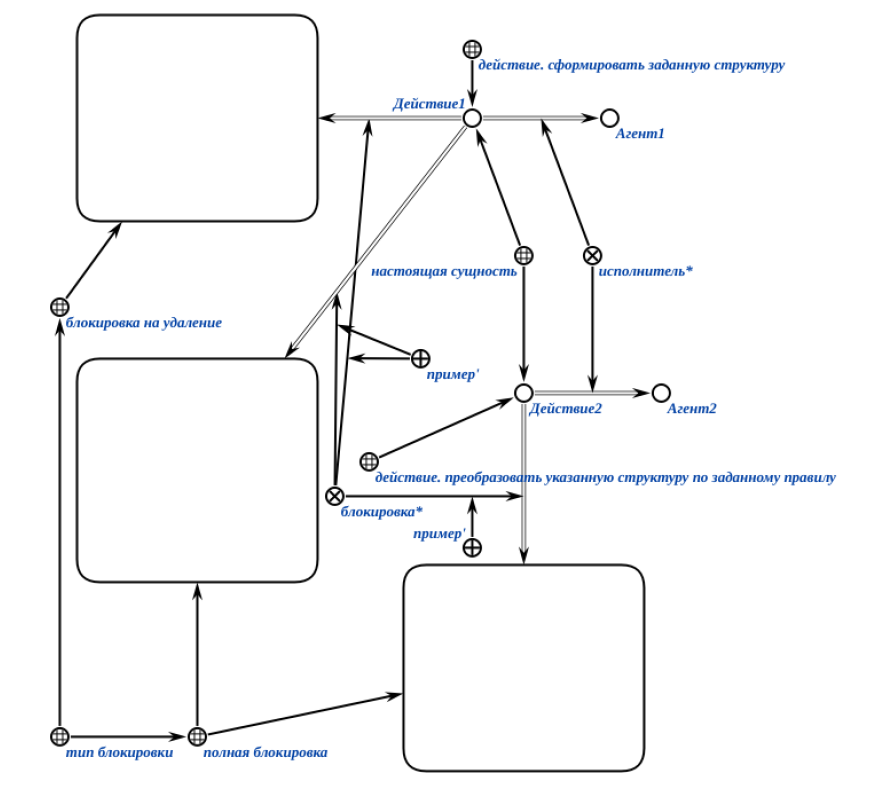
\includegraphics[scale=0.30]{./figures/sd_multiagent_processing/blocking_example.png}
		\caption{Пример использования блокировок}
	\end{figure}
\end{frame}
